\documentclass[12pt]{article}
\usepackage{graphicx}
\usepackage{mathptmx}
\usepackage[intlimits,centertags]{amsmath}
\usepackage{amssymb,amsfonts}
\usepackage[pdftex]{hyperref}
\usepackage{aas_macros}
\usepackage{enumerate}
\usepackage[symbol]{footmisc}
\usepackage{xfrac}
\usepackage[table,xcdraw]{xcolor}
\usepackage{sectsty}
\usepackage[normalem]{ulem}
\usepackage{setspace}
\usepackage{ragged2e}
\usepackage{combelow} 
\usepackage{etoolbox} 
\usepackage{cite}
\usepackage{fdsymbol}
\usepackage{pdfpages}
\usepackage[T1]{fontenc}
\usepackage{times}
\usepackage[compact]{titlesec}
\usepackage{geometry}
\geometry{letterpaper, portrait, margin=1in}
\usepackage[utf8]{inputenc}
\usepackage{enumitem,amssymb}
\usepackage{ragged2e}
\usepackage{wrapfig}
\newlist{thematic}{itemize}{8}
\setlist[thematic]{label=$\square$}
\usepackage{pifont}
\newcommand{\cmark}{\ding{51}}%
\newcommand{\xmark}{\ding{55}}%
\newcommand{\done}{\rlap{$\square$}{\raisebox{2pt}{\large\hspace{1pt}\cmark}}%
\hspace{-2.5pt}}
\newcommand{\wontfix}{\rlap{$\square$}{\large\hspace{1pt}\xmark}}
\renewcommand{\thefootnote}{\fnsymbol{footnote}}

\definecolor{darkgreen}{rgb}{0,0.5,0}
\definecolor{vermillion}{rgb}{0.89, 0.259, 0.204}


\newif\ifastrophysical
\astrophysicaltrue
\newcommand{\onlyastrophysical}[1] 
{
  \ifastrophysical
  #1 
  \fi
}

\newif\iffundamental
\fundamentalfalse
\newcommand{\onlyfundamental}[1] 
{
  \iffundamental
  #1 
  \fi
}


\definecolor{header_color}{HTML}{741a07}
\subsectionfont{\color{header_color}}
\renewcommand\refname{\color{header_color}References}


\begin{document}
\raggedright
\huge
Astro2020 Science White Paper \linebreak

Science Reach with a High-Elevation Radio Instrument, the Beamforming Elevated Array for COsmic Neutrinos \linebreak
\normalsize

\noindent \textbf{Thematic Areas:} \hspace*{60pt} $\square$ Planetary Systems \hspace*{10pt} $\square$ Star and Planet Formation \hspace*{20pt}\linebreak
$\square$ Formation and Evolution of Compact Objects \hspace*{31pt} $\square$ Cosmology and Fundamental Physics \linebreak
  $\square$  Stars and Stellar Evolution \hspace*{1pt} $\square$ Resolved Stellar Populations and their Environments \hspace*{40pt} \linebreak
  $\square$    Galaxy Evolution   \hspace*{45pt} $\checkmark$             Multi-Messenger Astronomy and Astrophysics \hspace*{65pt} \linebreak
  
\textbf{Principal Author:}

Name:	Stephanie Wissel
 \linebreak						
Institution:  California Polytechnic State University
 \linebreak
Email: swissel@calpoly.edu
 \linebreak
Phone:  805-756-7375
 \linebreak
 
\textbf{Co-authors:} (names and institutions)
  \linebreak

\textbf{Abstract  (optional):}

\normalsize
\pagebreak

\pagenumbering{arabic}

\pagebreak

Call Here:
https://sites.nationalacademies.org/cs/groups/depssite/documents/webpage/deps\_193135.pdf

FAQ Here: 
https://sites.nationalacademies.org/DEPS/Astro2020/DEPS\_192908

10 pages, including figures, but they can be links if necessary

\section{Key Science Goals and Objectives}
\color{blue}
The papers should summarize the most important scientific goals and objectives, justifying the timeliness of the scientific opportunities, and placing them in as broad a context as possible. We encourage the authors, where relevant, to reference Science White Papers submitted to the Survey (these are posted on the Astro2020 website, and may be referenced by author and title). Submitters may also make reference to web sites and other outside materials, but should strive to make this section as self-contained as possible.
\color{black}

High-energy observations of tau neutrinos have the unique capability to address outstanding questions in both astrophysics and fundamental physics, as outlined in three white papers~\cite{Astro2020_fundamental, Astro2020_astrophysics, Astro2020_blazars}. The goals of BEACON, a 100-PeV scale neutrino observatory are:
\begin{enumerate}
	\item Extending the cosmic neutrino spectrum to higher energies	\item Unambiguous detection of an extragalactic source of cosmic neutrinos
 	\item Multi-messenger observations enabled by the highest energy neutrinos at mid-latitudes
	\item Tau fraction can point to different acceleration mechanisms at the sources and possibly beyond-the-standard model physics
\end{enumerate}

%% Make this paragraph sexier
%% This is why we want to extend to higher energies from a multi-messenger 
\textbf{The High Energy End of the Cosmic Neutrino Spectrum} Cosmic neutrino production depends on the assumed acceleration mechanism and source types, both of which are informed by observations by the IceCube neutrino observatory in a lower energy range from 100 TeV to 10 PeV. IceCube has reported on three main analysis of the cosmic neutrino spectrum. Through-going muon neutrinos indicate a hard spectrum with an index of $E^{-2.13\pm0.13}$. Since the neutrino-nucleon cross section grows roughly as $E^{2}$, fully efficient detectors should expect a constant rate of neutrinos across their energy band. However, analyses using the all-flavor and high-energy events contained entirely in the detection tor favor a softer spectral indices of $\sim2.5$. 

The difference in measured spectral indices can be attributed to the energy threshold of the different analyses, meaning that as with photons, the universe mapped in neutrinos is complex. Different sources contribute the neutrino sky and only through improved event statistics, improved angular resolution, extensions to higher energies, and deeper understanding of the flavor composition can we build a complete map of the neutrino sky. 


Active galactic nuclei, pulsars, gamma-ray bursts, and galaxy clusters are all implicated as possible accelerators of ultra-high energy cosmic rays that achieve energies greater than $10^{21}$~eV. The origin of these cosmic rays has confounded the field for decades in part because cosmic rays up to a certain rigidity are unreliable narrators. Such accelerators pump cosmic rays (protons and other nuclei) into the local environment where through $pp$ and $p\gamma$ interactions they can deposit energy into neutrinos, gamma rays, and secondary cosmic rays. Cosmic neutrinos can thus identify the sources of the highest energy particle acceleration in the universe.


Cosmogenic neutrinos are additionally expected at energies above 1 EeV from the interactions of the highest energy cosmic rays with background photons during cosmic ray propagation. Because cosmic rays interact with photon backgrounds within a mean free path of hundreds of megaparsecs and gamma rays are absorbed by the extra galactic background light, cosmogenic neutrinos may provide the only particle probe of the high energy end of the universe at gigaparsec length scales. The long baselines and high energies allow us to probe fundamental physics in otherwise inaccessible energy regimes and length scales~\cite{astro2020_fundamental}.

Tau neutrinos also have important implications for the new field of neutrino astronomy with TeV-PeV scale neutrinos. Although revolutionary in their discovery, neutrinos produced directly in the cores of extreme astrophysical environments come from as-of-yet unknown sources. By targeting the energy range where the PeV neutrinos and cosmogenic neutrino flux overlap, this project will lay the groundwork for revealing the physics driving the astrophysical PeV accelerators in addition to the cosmological evolution of the high-energy universe.
	
Two white papers determined the requirements on $>100$ PeV-scale tau neutrino observatories to be \cite{Astro2020_fundamental, Astro2020_astrophysics}:
\begin{itemize}
	\item Energy spectral resolution of half-decade or better to measure cross-sections and spectral features associated with different acceleration mechanisms and BSM physics
	\item High event statistics, of approximately 100 neutrinos of a given flavor
	\item Flavor identification of 40\% or better
	\item Sub-degree pointing resolution
\end{itemize}


With BEACON, we expect to achieve sub-degree scale pointing and half-decade energy resolution. We expect to either observe as much as 10-30 tau neutrinos over a five year period or place limits on the maximum energy of cosmic ray accelerators and the extension to the diffuse IceCube neutrino flux.  Since the number of observed neutrinos is model dependent. 

\section{Technical Overview}
\color{blue}
The team should provide a description of the technical aspects of the pursuit, including a description of the essential performance parameters for achieving the project's science goals.

For ground-based activities/projects, papers should describe the telescope or observatory architecture, key performance requirements, technical requirements, anticipated site and infrastructure requirements, as well as any public/private partnerships.
\color{black}

BEACON targets the sources and flux of tau neutrino by searching for Earth-skimming, upgoing tau neutrinos. As shown in Fig.~\ref{fig:concept}, BEACON consists of a radio interferometer located on a high elevation mountain. Each station monitors an independent portion of the valley for tau leptons exiting the Earth after being produced by tau neutrinos through a charged current interaction inside the Earth. The sensitivity of each station is maximized by placing the stations on mountain prominences at least 2~km above the valley. 

\begin{figure}[htbp]
\begin{center}
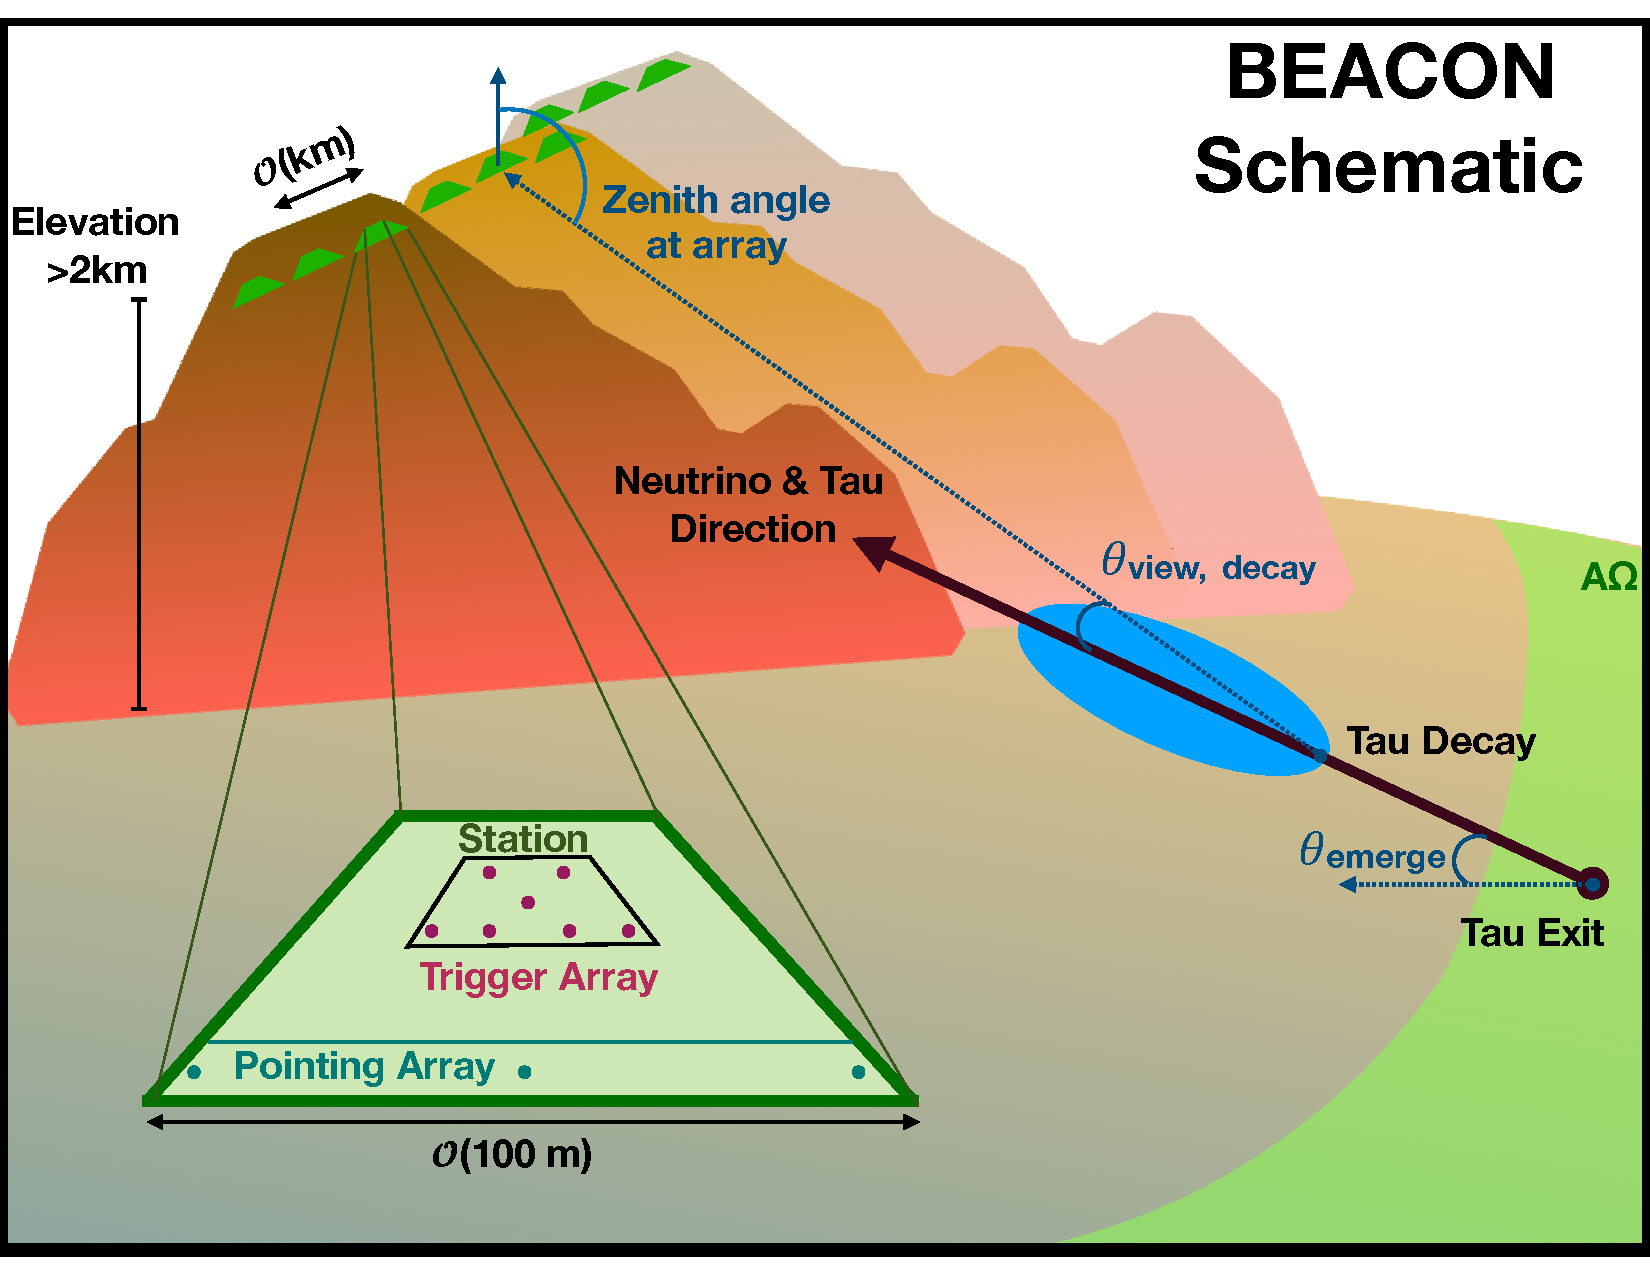
\includegraphics[width=0.7\textwidth]{figures/BEACON_ICRC_Concept.pdf}
\caption{Concept of a high-elevation mountaintop detector.}
\label{fig:concept}
\end{center}
\end{figure}

\subsection{BEACON Architecture}

A promising technique for detecting cosmogenic tau neutrinos looks for radio-frequency (RF) radiation from the particle showers they initiate in the Earth's atmosphere. The signature of a tau neutrino would be an upcoming broadband radio spark produced by a tau lepton decay in air. Because this channel is inaccessible to electron or muon neutrino detection, tau neutrinos present a unique opportunity for studying the neutrino flavor content of the highest energy neutrinos. By maximizing the single detector exposure and by using inexpensive instrumentation deployed in hospitable environments, a high-elevation mountaintop radio detector is a scalable solution to achieving the enormous effective areas necessitated by the expected neutrino flux at $>100$~PeV. 

A key aspect of the BEACON concept is the use digital, time-domain interferometry which observes the signal from an air shower on multiple antennas, and coherently delays and sums the signals. Interferometric techniques can improve the angular reconstruction of the signals and enhances background rejection, both at the trigger level and in rejecting backgrounds at the analysis level. 

BEACON detectors can be placed at multiple sites throughout the world to achieve high point source sensitivity and full sky coverage required for searches for neutrinos from explosive transients expected from supernova, gamma ray bursts, blazar flares, and other targets of multi-messenger astrophysics. Different sites view different regions of the sky, and detectors located at mid-latitudes achieve broader sky coverage than those in polar regions. Full sky coverage or a deep exposure towards the galactic center could be achieved through a a thoughtfully designed global network of high-elevation radio instruments. 

This detector design is still in the conceptual stage where different choices for the detector design are being weighted against cost, logistical challenges, and performance. We outline the key performance parameters and the trade-offs associated with them below.

\subsection{Performance Requirements}
\begin{enumerate}
\item Elevation
\item Thresholds and Duty Cycle
\item Angular Resolution
\item Backgrounds
\end{enumerate}

The acceptance of a single station to an isotropic tau neutrino flux depends on the elevation of the detector and the combined probabilities that a tau lepton will exit the Earth, that it will decay before reaching the detector, and that the receiver will register the radio signal. 

A first order estimate of the acceptance of a high-elevation radio receiver, shown in Fig.~\ref{fig:crude_estimate}(left), gives insight into how the geometry of this design enhances the sensitivity of each station. Motloch, et al give an analytical estimate of the geometric aperture of a high-elevation, $h$, receiver~\cite{Motloch2014}. 
%The probability that a tau lepton will exit, $P_{exit}$ was calculated assuming Standard model interaction cross sections and energy losses by Alvarez-Mu\~niz, et al~\cite{Alvarez-Muniz2018} to be uniform at 100 PeV up to emergence angles of 10$^{\circ}$ and more concentrated towards Earth-skimming angles at higher energies.
A tau lepton emerges as the result of a charged current interaction of the original tau neutrino, the probability, $P_{exit}$ of which was calculated by  Alvarez-Mu\~niz, et al~\cite{Alvarez-Muniz2018}.The tau will decay within a a decay length $L_{decay} = 49$~km($E_{\tau}$/EeV), such that tau leptons emerging at the horizon with energies below 3 EeV with always decay before reaching the mountain ridge. We assume that all events initiated within a few degrees (1-3$^{\circ}$) view angle of the neutrino direction are detected by the detector, based on the radio beam pattern of an air shower. Because the geometric aperture grows as $h^{1.5}$, the total acceptance increases by a factor of 7 going from 1~km to 2~km and by an additional factor of 2.5 going from 2~km to 4~km. 

%\begin{table}[htbp]
 % \centering
 % \begin{tabular}{@{} cccccc @{}}
  %\toprule
 %   Elevation (km) & Aperture (km$^2$ sr) & $P_{exit}(10^{17}$ eV) & $P_{exit}(10^{18}$ eV) & $A\Omega(10^{17}$~eV) & $A\Omega(10^{18}$~eV)\\ 
    %\midrule
  %  1 & 0.1 & 8e-4 & 8e-3 & 8e-5 & 8e-2 \\
  %  2 & 0.7 & 8e-4 & 8e-3 & 5.6e-4 & 5.6e-3 \\ 
  %  3 & 1 & 8e-4 &  8e-3 & 1e-4 & 8e-3  \\ 
    %\bottomrule
 % \end{tabular}
  %\caption{Rough order of magnitude estimates for the acceptance of a high elevation detector based on the geometric acceptance formula of Motloch, Hollon, Priviter 2014. We assume a factor of $1/3$ to account for an expected 120$^\circ$ field of view. For each energy, we have multiplied the geometric acceptance estimate by the peak $P_\mathrm{exit}$ values of Alvarez-Mu\~niz et al. 2018.}
  %\label{fig:crude_estimate}
%\end{table}

The radio beam expected from tau lepton air showers drives the design of the high-elevation antennas in terms of their frequency band and gain. The radio signal is broadband from $\sim$10~MHz to 1~GHz, meaning that various choice can be made about the optimal antenna and frequency band chosen. For instance, as shown in Fig.~\ref{fig:crude_estimate}(right), a 30-80~MHz beam is broad, covering a wide range of view angles. Alternatively, the beam in the 200-1200~MHz frequency band can be more strongly peaked at Cherenkov angle, as shown in Fig.~\ref{fig:crude_estimate}(right). 

Short dipole antennas are readily available in the 30-80~MHz band, typically with gains of 1.8~dBi or better. At higher frequencies, horn antennas and log-periodic dipole antennas can cover a broader range of frequencies and with higher gains. Typical antennas can range from 200~MHz to 1~GHz with gains between 6~dBi and 10~dBi. Incoherent radio backgrounds are dominated by the galactic sky noise in the lower frequency band and by thermal emission from the ground in the higher frequencies. Ultimately, because the acceptance (see Fig.~\ref{fig:acceptance} differs by at most a factor of 2 for the two frequency bands considered, the radio backgrounds local to the chosen sites and the angular resolution requirements should determine the final choice of frequency band in the design.

\begin{figure}[!h]
{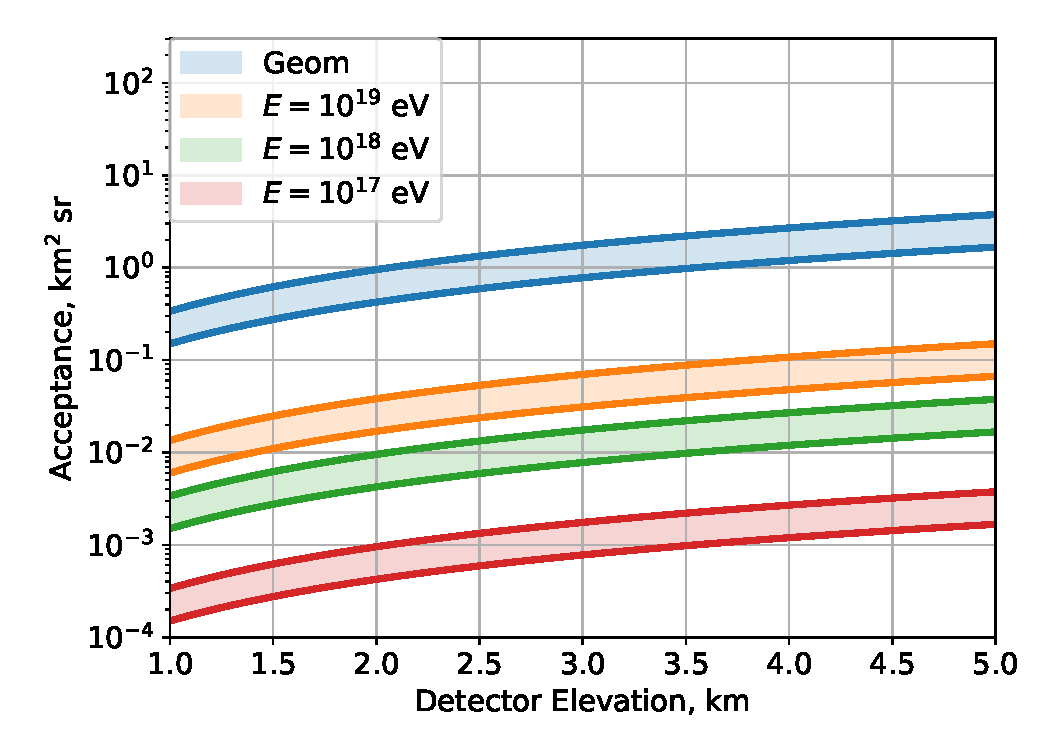
\includegraphics[width=0.45\textwidth]{figures/Crude_Estimate.pdf}}
{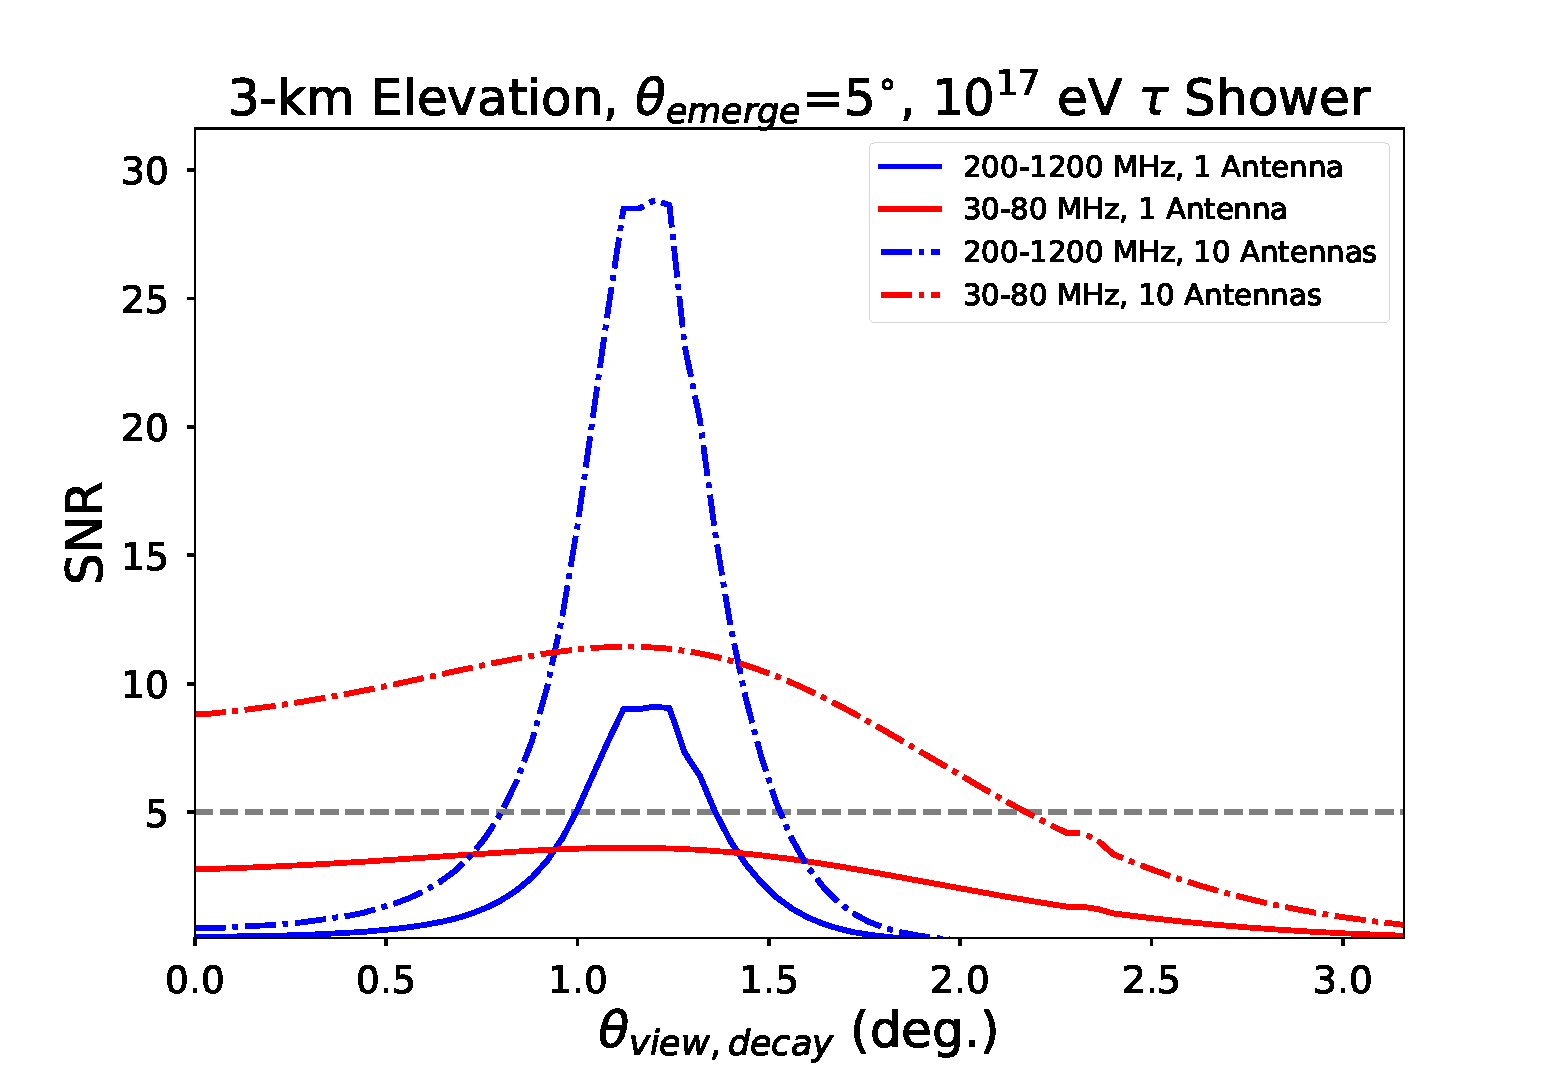
\includegraphics[width=0.48\textwidth]{figures/SNR_example_emerge5deg_10antenna.pdf}}
%this figure was created in ARW's laptop Desktop/BEACON_sim_new/CrudeEstimate.ipynb
\caption{Left: Order of magnitude estimates for the acceptance of a high elevation detector based on the geometric acceptance formula of Motloch, Hollon, Priviter 2014. We assume a factor of $1/3$ to account for an expected 120$^\circ$ field of view. For each energy, we have multiplied the geometric acceptance estimate by the peak $P_\mathrm{exit}$ values of Alvarez-Mu\~niz et al. 2018. Right: A $10^{17}$~eV $\tau$ shower emerging at a 5$^{\circ}$ and decaying at the exit point generates a radio beam pattern shown here as the SNR versus $\theta_{view,decay}$.  The radio emission is filtered in the 30-80 MHz (red) and 200-1200 MHz bands (blue) for 1 antenna (solid) and 10 phased antennas (dot-dashed).   }
\label{fig:crude_estimate}
\end{figure}



The optimal design of a high elevation radio interferometer depends on several factors shown on the right in Fig.~\ref{fig:acceptance} including the detector elevation (top), the effective gain of the phased array (middle), and the average trigger threshold on the beam (bottom). The acceptance ratios are referenced to a design of a single BEACON station composed of 7 phased antennas each with a gain of 1.8 dBi and a frequency band of 30-80 MHz placed at an elevation of 3 km with a 5$\sigma$ threshold on the beam.

%1.	The VHF design has a higher acceptance for E>1017.5 eV, while the UHF design yields a lower threshold.
%2.	The station acceptance linearly increases with the number of antennas up to 10 antennas, but sub-linearly above that (see Fig. 3). When increasing the number of stations, however, the acceptance increases linearly regardless of antenna number, assuming the visible volume of each station is independent.
%3.	The number of expected neutrinos from standard cosmogenic models increases linearly with the elevation of the station up to 3 km, while power laws (such as the IceCube flux) or models with cutoffs E<1018 eV are largely insensitive to elevation changes above 1 km. 
%4.	The number of expected neutrinos is insensitive to whether it overlooks rock or ocean, provided it has view out to the horizon. Ocean may still be preferable; however, because manmade noise is more prevalent in the valleys near high-elevation land-locked mountains than over the deep ocean.
Informed by these results, the reference design for the BEACON prototype is a single station with 10 phased antennas at 3 km altitude. Using ten phased antennas in a single station has the benefit of being able to form multiple beams that can help with not only direction reconstruction, but also with reducing backgrounds from anthropogenic sources. Upon demonstration of its feasibility as a neutrino detector, the BEACON detector could be expanded to include 10 stations sited either along the same mountain ridge or at multiple sites around the world, thereby scaling up to constrain the UHE neutrino flux and achieve full sky coverage using a technique complementary to IceCube and IceCube-Gen2. Multiple stations along the same ridge could act as a veto for man-made radio transients such as air planes. 


\begin{figure}[hbtp]
\begin{center}
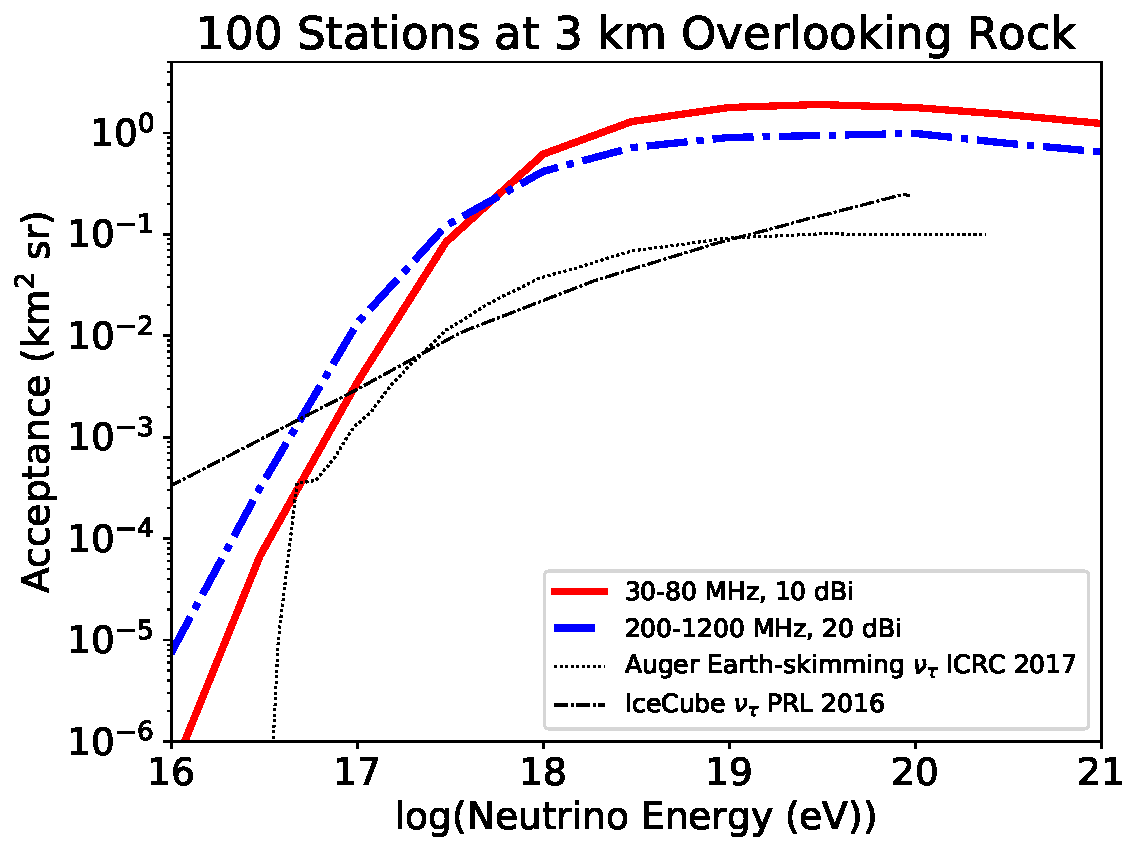
\includegraphics[width=0.54\textwidth]{figures/acceptance_100stations_energyssampling}
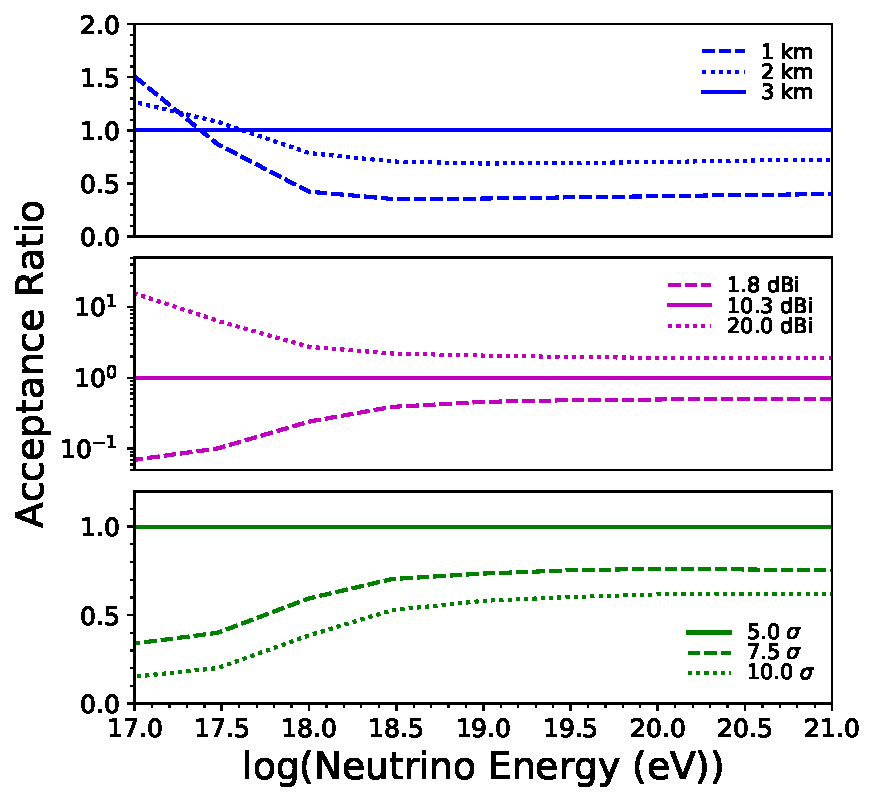
\includegraphics[width=0.45\textwidth]{figures/acceptanceratio_100stations_energyssampling_study}
\caption{(left) The acceptance of BEACON in two different frequency bands compared with the acceptance of PAO to Earth-skimming tau neutrinos and IceCube to tau neutrinos. The designs assume 100 stations at an elevation of 3 km. Each station comprises 7 antennas in the 30-80 MHz range and 10 antennas in the 200-1200 MHz range, both with a threshold of 5$\sigma$. (right) The ratio of the acceptance of a 30-80 MHz detector for different elevations (top), phased array gains (middle), and trigger thresholds (bottom) relative to the reference design. }
\label{fig:acceptance}
\end{center}
\end{figure}

\begin{figure}[tbhp]
\begin{center}
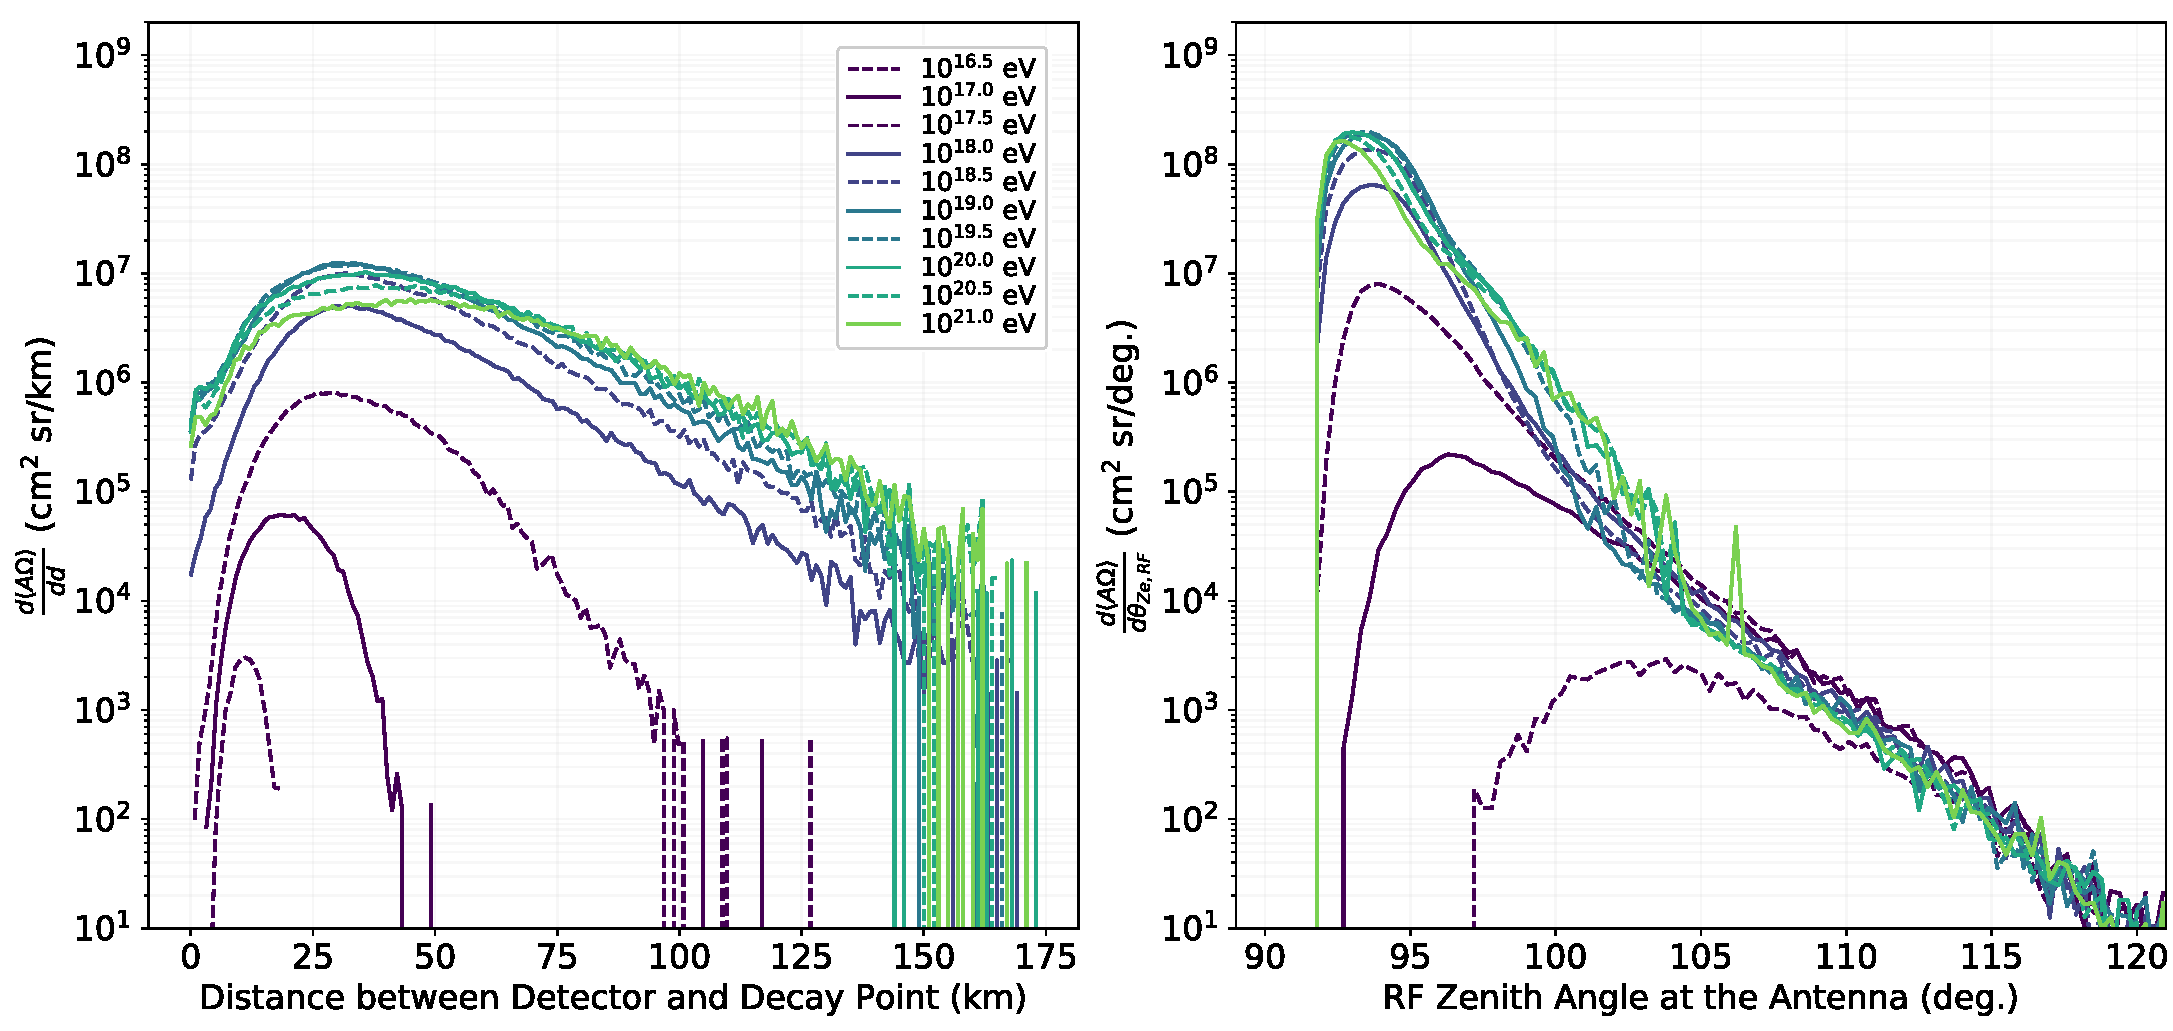
\includegraphics[width=\textwidth]{figures/diffacceptance_30-80MHz_refdesign}
\caption{Differential acceptance of the BEACON reference station to isotropoic tau neutrino flux shows the predominant distances between the decay point and the detector (left) and the zenith angles measured at the array (right) for various energies.}
\label{fig:diffaccep}
\end{center}
\end{figure}


\subsection{Site and Infrastructure Requirements}


\section{Technology Drivers}
\color{blue}
If the pursuit requires new technologies, the paper should identify and describe them, along with an outline of technology maturation plans and timescales.
\color{black}

\section{Organization, Partnerships, and
Current Status} 
\color{blue}
All pursuits should describe the participating organizations, any planned partnerships, and their current status.
\color{black}

\section{Schedule} 
\color{blue}
The team should outline the development and operations schedule. The schedule should also indicate the operational lifetime of the pursuit.
\color{black}

\section{Cost Estimates}
\color{blue}
 The team should provide any cost estimates that have been developed for the current version of the pursuit. 
 \color{black}

\pagebreak
\textbf{References}



\end{document}

